\documentclass[10pt, a4paper]{ctexart}
\usepackage[margin=1in]{geometry}
\usepackage{bm}
\usepackage{amsmath}
\usepackage{graphicx}
\usepackage{float}
\usepackage{listings}
\usepackage{tikz}

\renewcommand{\figurename}{Figure.}
\renewcommand{\tablename}{Table.}

\begin{document}
\title{Assignment 2}
\date{}
\author{}
\maketitle

\section{Tensorflow Softmax}
{\bf{(a)}} See file q1\_softmax.py\par
{\bf{(b)}} See file q1\_softmax.py\par
{\bf{(c)}} The purpose of placeholder is to hold our input data, and the purpose of feed dictionaries is to feed input values to placeholders. See implementation in file q1\_classifier.py\par
{\bf{(d)}} See file q1\_classifier.py\par
{\bf({e})} See file q1\_classifier.py. After the model's {\emph{train\_op}} is called, the prediction {\emph{y\_hat}} is computed in the forward propagation and the gradient of loss with respect to {\emph{W}} and {\emph{b}} is computed during the back propagation. The variable {\emph{W}} and {\emph{b}} will be changed.\par

\section{Neural Transition-Based Dependency Parsing}
{\bf{(a)}} The parsing procedure is as follows:
\begin{table}[H]
    \centering
    \resizebox{\textwidth}{29mm}{
    \begin{tabular}{l|l|l|l}
        stack&buffer&new dependency&transition\\
        \hline
        [ROOT]&[I, parsed, this, sentence, correctly]&&Initial Configuration\\\relax
        [ROOT, I]&[parsed, this, sentence, correctly]&&SHIFT\\\relax
        [ROOT, I, parsed]&[this, sentence, correctly]&&SHIFT\\\relax
        [ROOT, parsed]&[this, sentence, correctly]&parsed$\rightarrow$I&LEFT-ARC\\\relax
        [ROOT, parsed, this]&[sentence, correctly]&&SHIFT\\\relax
        [ROOT, parsed, this, sentence]&[correctly]&&SHIFT\\\relax
        [ROOT, parsed, sentence]&[correctly]&sentence$\rightarrow$this&LEFT-ARC\\\relax
        [ROOT, parsed]&[correctly]&parsed$\rightarrow$sentence&RIGHT-ARC\\\relax
        [ROOT, parsed, correctly]&[]&&SHIFT\\\relax
        [ROOT, parsed]&[]&parsed$\rightarrow$correctly&RIGHT-ARC\\\relax
        [ROOT]&[]&ROOT$\rightarrow$parsed&RIGHT-ARC\\
    \end{tabular}
    }
    \caption{Parsing Procedure}
\end{table}
{\bf{(b)}} A sentence containing $n$ words will be parsed in $2\times n$ steps. This is true because every word will be shifted into the stack once, and will be removed from the stack once, therefore, the total number of steps is $2\times n$.\par
{\bf{(c)}} See file q2\_parser\_transitions.py\par
{\bf{(d)}} See file q2\_parser\_transitions.py\par
{\bf{(e)}} See file q2\_initialization.py\par
{\bf{(f)}} The constant $\gamma$ can be expressed as:
\begin{align*}
    \gamma = \frac{1}{1-p_{drop}}
\end{align*}
This is true because the expected value of $h_{drop}$ is $(1-p_{drop})h$.\par
{\bf{(g)}}\par
{\hspace{10pt}}(i) By using $m$, the amount of steps we take at each update will now become the running average of gradients of all times. And the current gradient calculated only contribute a little to the $m$, therefore it is more stable and can stop the updates from varying too much.\par
{\hspace{10pt}}(ii) The parameters that have smaller gradient will get larger updates. This helps the learning because it will smooth the updates we make and try to update all parameters equally.\par
{\bf{(h)}} See file q2\_parser\_model.py and predictions in file q2\_test.predicted.pkl\par
The best UAS my model achieves on the dev set is $88.70$, and the UAS achieves on the test set is $88.87$.

\section{Recurrent Neural Networks: Language Modeling}
{\bf{(a)}}\par
{\hspace{10pt}}(i) Assuming $k$ is the right word at position $t+1$, then we have:
\begin{align*}
    \frac{1}{\exp\bigg(-J^{(t)}(\theta)\bigg)}&=\frac{1}{\exp\bigg(\sum_{j=1}^{|V|}y_j^{(t)}\log \hat{y}_j^{(t)}\bigg)}\\
    &=\frac{1}{\hat{y}_k^{t}}\\
    &=\frac{1}{\bar{P}({\bm{x}}_{pred}^{(t+1)}={\bm{x}}^{(t+1)}|{\bm{x}}^{(t)},\dots,{\bm{x}}^{(1)})}\\
    &={\rm{PP}}\bigg(y^{(t)},\hat{y}^{(t)}\bigg)\\
\end{align*}\par
{\hspace{10pt}}(ii) By using the result above, we have:
\begin{align*}
    \log\bigg(\prod_{t=1}^TPP(y^{(t)},\hat{y}^{(t)})\bigg)^{1/T}&=\log\Bigg(\frac{1}{\exp\big(-\sum_{t=1}^TJ^{(t)}(\theta)\big)}\Bigg)^{1/T}\\
    &=\frac{1}{T}\sum_{t=1}^TJ^{(t)}(\theta)
\end{align*}
For any positive function, minimizing its logarithm is equivalent to minimizing f itself, therefore minimizing the geometric mean perplexity is the same as minimizing the function above, which is the arithmetic mean cross-entropy loss.\par
{\hspace{10pt}}(iii) For a single word, the perplexity is $|V|$. When $|V|=10000$, the cross-entropy loss is $\log 10000\approx 9.21$\par
{\bf{(b)}} Let's define:
\begin{align*}
    &z^{(t)} = W_hh^{(t-1)}+W_ee^{(t)}+b_1\\
    &\theta^{(t)}=Uh^{(t)}+b_2\\
    &\delta_1^{(t)}=\frac{\partial J}{\partial \theta^{(t)}}\\
    &\delta_2^{(t)}=\frac{\partial J}{\partial z^{(t)}}=\delta_1^{(t)}\frac{\partial \theta^{(t)}}{\partial h^{(t)}}\frac{\partial h^{(t)}}{\partial z^{(t)}}
\end{align*}
We then have:
\begin{align*}
    &\delta_1^{(t)}=\hat{y}^{(t)}-y^{(t)}\\
    &\frac{\partial J^{(t)}}{\partial U}=\delta_1^{(t)}{h^{(t)}}^T\\
    &\frac{\partial J^{(t)}}{\partial h^{(t)}}=U^T\delta_1^{(t)}\\
    &\delta_2^{(t)}=(U^T\delta_1^{(t)})\odot\big(z^{(t)}\odot(1-z^{(t)})\big)\\
    &\frac{\partial J^{(t)}}{\partial W_e}\vert_{(t)}=\delta_2^{(t)}{e^{(t)}}^T\\
    &\frac{\partial J^{(t)}}{\partial W_h}\vert_{(t)}=\delta_2^{(t)}{h^{(t-1)}}^T\\
    &\frac{\partial J^{(t)}}{\partial h^{(t-1)}}={W_h}^T\delta_2^{(t)}
\end{align*}\par
{\bf{(c)}}
\begin{figure}[H]
    \centering
    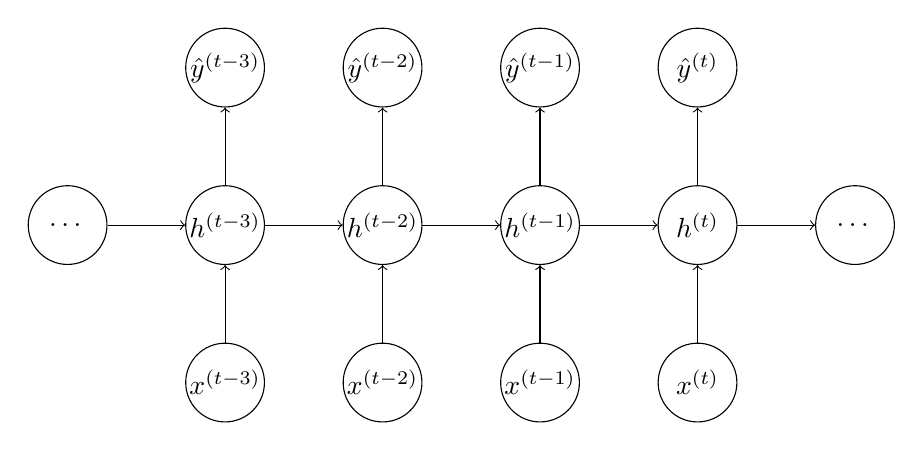
\begin{tikzpicture}
        \node[draw, circle, minimum size=1cm, inner sep=0pt] (h0) at (-2,0) {$\dots$};
        \node[draw, circle, minimum size=1cm, inner sep=0pt] (h1) at (0,0) {$h^{(t-3)}$};
        \node[draw, circle, minimum size=1cm, inner sep=0pt] (y1) at (0,2) {$\hat{y}^{(t-3)}$};
        \node[draw, circle, minimum size=1cm, inner sep=0pt] (x1) at (0,-2) {$x^{(t-3)}$};
        \node[draw, circle, minimum size=1cm, inner sep=0pt] (h2) at (2,0) {$h^{(t-2)}$};
        \node[draw, circle, minimum size=1cm, inner sep=0pt] (y2) at (2,2) {$\hat{y}^{(t-2)}$};
        \node[draw, circle, minimum size=1cm, inner sep=0pt] (x2) at (2,-2) {$x^{(t-2)}$};
        \node[draw, circle, minimum size=1cm, inner sep=0pt] (h3) at (4,0) {$h^{(t-1)}$};
        \node[draw, circle, minimum size=1cm, inner sep=0pt] (y3) at (4,2) {$\hat{y}^{(t-1)}$};
        \node[draw, circle, minimum size=1cm, inner sep=0pt] (x3) at (4,-2) {$x^{(t-1)}$};
        \node[draw, circle, minimum size=1cm, inner sep=0pt] (h4) at (6,0) {$h^{(t)}$};
        \node[draw, circle, minimum size=1cm, inner sep=0pt] (y4) at (6,2) {$\hat{y}^{(t)}$};
        \node[draw, circle, minimum size=1cm, inner sep=0pt] (x4) at (6,-2) {$x^{(t)}$};
        \node[draw, circle, minimum size=1cm, inner sep=0pt] (h5) at (8,0) {$\dots$};

        \draw[->] (h1) edge (y1);
        \draw[->] (x1) edge (h1);
        \draw[->] (h1) edge (h2);
        \draw[->] (h2) edge (y2);
        \draw[->] (x2) edge (h2);
        \draw[->] (h2) edge (h3);
        \draw[->] (h3) edge (y3);
        \draw[->] (x3) edge (h3);
        \draw[->] (h3) edge (h4);
        \draw[->] (h4) edge (y4);
        \draw[->] (x4) edge (h4);
        \draw[->] (h0) edge (h1);
        \draw[->] (h4) edge (h5);
    \end{tikzpicture}
    \caption{The "Unrolled" Network for 3 Timesteps}
\end{figure}\par
The gradients can be calculated as follows:
\begin{align*}
    &\frac{\partial J^{(t)}}{\partial e^{(t-1)}}={W_e}^T\bigg(\gamma^{(t-1)}\odot\big(z^{(t-1)}\odot(1-z^{(t-1)})\big)\bigg)\\
    &\frac{\partial J^{(t)}}{\partial W_e}\vert_{(t-1)}=\delta_2^{(t)}{e^{(t)}}^T+\bigg(\gamma^{(t-1)}\odot\big(z^{(t-1)}\odot(1-z^{(t-1)})\big)\bigg){e^{t-1}}^T\\
    &\frac{\partial J^{(t)}}{\partial W_h}\vert_{(t-1)}=\delta_2^{(t)}{h^{t-1}}^T+\bigg(\gamma^{(t-1)}\odot\big(z^{(t-1)}\odot(1-z^{(t-1)})\big)\bigg){h^{t-2}}^T\\
\end{align*}\par
{\bf{(d)}} Given $h^{(t-1)}$, first we need $O(d\times |V|+D_h\times D_h+D_h\times d+|V|\times D_h)$ to do forward propagation. Then we need $O(|V|\times D_h+|V|\times D_h+D_h\times d+D_h\times D_h+D_h\times D_h)$ to do back propagation.\par
{\bf{(e)}} The total number of operations we need to do forward propagation is simply $O(T\times \big(d\times |V|+D_h\times D_h+D_h\times d+|V|\times D_h\big))$, and the total number of operations we need to do back propagation is:
\begin{align*}
    O(3\times T\times\big(|V|\times D_h+D_h\times d+D_h\times D_h\big)) 
\end{align*}\par
{\bf{(f)}} The term $|V|\times D_h$ is likely to be the largest if we use a large corpus, and it's from the output layer (the one that calculates the output according to current hidden state) of the RNN.
\end{document}